\documentclass{article}
\usepackage[T1]{fontenc}
\usepackage{lmodern}
\usepackage{graphicx}
\usepackage{amsmath,amssymb}
\usepackage[a4paper,margin=2cm]{geometry}
\usepackage[absolute,overlay]{textpos}
\setlength{\TPHorizModule}{1mm}
\setlength{\TPVertModule}{1mm}
\usepackage[indonesian]{babel}
\usepackage{hyperref}
\setlength{\emergencystretch}{2em}
% unit: Halaman 38

\begin{document}

% === Halaman 38 (llm) ===

\section*{Mode CFB}

\vspace{60mm}

\textbf{Enkripsi:}
\[ C_j = P_j \oplus MSB_s(E_K(X_j)) \]
\[ X_{j+1} = LSB_{b-s}(X_j) \parallel C_i \]

\textbf{Dekripsi:}
\[ P_j = C_i \oplus MSB_s(E_K(X_j)) \]
\[ X_{j+1} = LSB_{b-s}(X_j) \parallel C_i \]

\vspace{10mm}

Mode CFB mengoperasikan \textbf{block cipher seperti stream cipher!!}

% deskripsi: Diagram blok proses enkripsi Mode CFB yang menunjukkan penggunaan IV, register geser, operasi enkripsi, dan XOR dengan plaintext untuk menghasilkan ciphertext.
% bbox normalisasi: [0.0120, 0.1270, 0.4970, 0.6370]
\begin{textblock*}{101.85mm}(2.52mm,37.72mm)
\noindent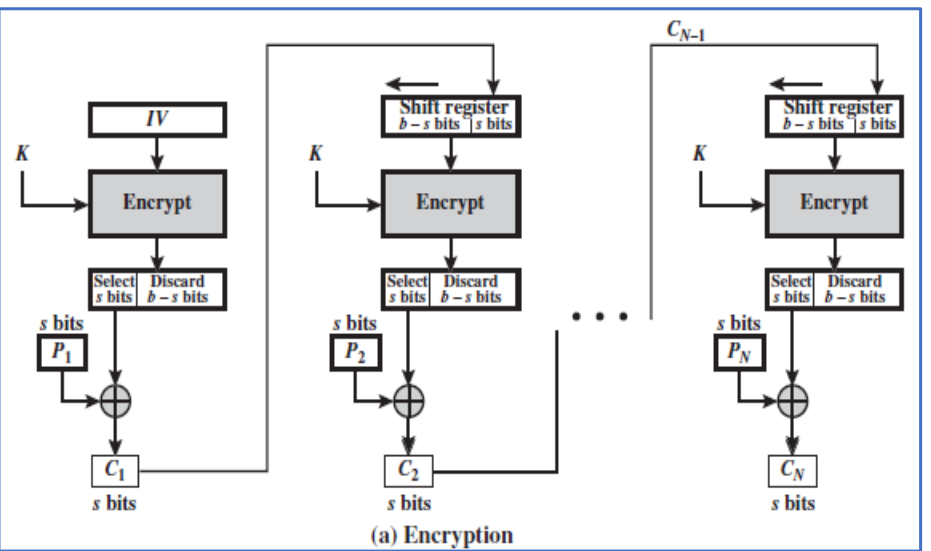
\includegraphics[width=101.85mm,height=151.47mm]{../../images/llm/page_038_img_01.png}%
\end{textblock*}

% deskripsi: Diagram blok proses dekripsi Mode CFB yang menunjukkan proses pemulihan plaintext menggunakan ciphertext dan output dari cipher block yang terenkripsi.
% bbox normalisasi: [0.5030, 0.1270, 0.9880, 0.6370]
\begin{textblock*}{101.85mm}(105.63mm,37.72mm)
\noindent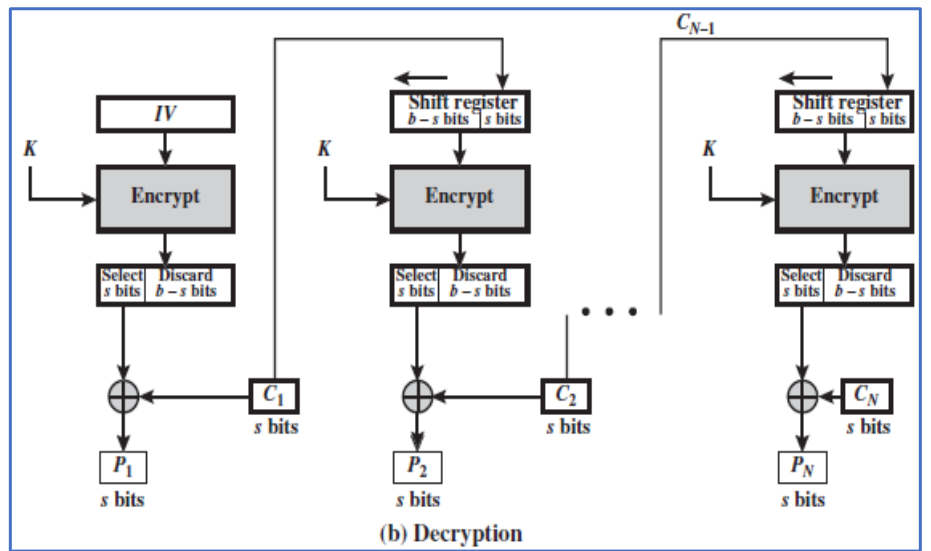
\includegraphics[width=101.85mm,height=151.47mm]{../../images/llm/page_038_img_02.png}%
\end{textblock*}

\end{document}
